\documentclass[a4paper,12pt]{article}
\usepackage{fullpage}
\usepackage[british]{babel}
\usepackage[T1]{fontenc}
\usepackage{amsmath}
\usepackage{amssymb}
\usepackage{amsthm} \newtheorem{theorem}{Theorem}
\usepackage{color}
\usepackage{float}
\usepackage{alltt}
\usepackage{listings}
%\usepackage{algorithm}
\usepackage[noend]{algorithm2e}
%\usepackage{algorithmicx}
\usepackage{subfig}
\lstset{% parameters for all code listings
	language=Python,
	frame=single,
	basicstyle=\small,  % nothing smaller than \footnotesize, please
	tabsize=2,
	numbers=left,
	framexleftmargin=2em,  % extend frame to include line numbers
	%xrightmargin=2em,  % extra space to fit 79 characters
	breaklines=true,
	breakatwhitespace=true,
	prebreak={/},
	captionpos=b,
	columns=fullflexible,
	escapeinside={\#*}{\^^M}
}


\usepackage{fancyvrb}
\DefineVerbatimEnvironment{code}{Verbatim}{fontsize=\small}
\DefineVerbatimEnvironment{example}{Verbatim}{fontsize=\small}

\usepackage{tikz} \usetikzlibrary{trees}
\usepackage{hyperref}  % should always be the last package

% useful colours (use sparingly!):
\newcommand{\blue}[1]{{\color{blue}#1}}
\newcommand{\green}[1]{{\color{green}#1}}
\newcommand{\red}[1]{{\color{red}#1}}

% useful wrappers for algorithmic/Python notation:
\newcommand{\length}[1]{\text{len}(#1)}
\newcommand{\twodots}{\mathinner{\ldotp\ldotp}}  % taken from clrscode3e.sty
\newcommand{\Oh}[1]{\mathcal{O}\left(#1\right)}

% useful (wrappers for) math symbols:
\newcommand{\Cardinality}[1]{\left\lvert#1\right\rvert}
%\newcommand{\Cardinality}[1]{\##1}
\newcommand{\Ceiling}[1]{\left\lceil#1\right\rceil}
\newcommand{\Floor}[1]{\left\lfloor#1\right\rfloor}
\newcommand{\Iff}{\Leftrightarrow}
\newcommand{\Implies}{\Rightarrow}
\newcommand{\Intersect}{\cap}
\newcommand{\Sequence}[1]{\left[#1\right]}
\newcommand{\Set}[1]{\left\{#1\right\}}
\newcommand{\SetComp}[2]{\Set{#1\SuchThat#2}}
\newcommand{\SuchThat}{\mid}
\newcommand{\Tuple}[1]{\langle#1\rangle}
\newcommand{\Union}{\cup}
\usetikzlibrary{positioning,shapes,shadows,arrows}


\title{\textbf{Separation of Voronoi Areas}}

\author{Martin Gebert, Sascha Schreckenbach, Jonathan Sharyari}  % replace by your name(s)

%\date{Month Day, Year}
\date{\today}

\begin{document}

\maketitle

\section{Abstract - do we need one?}
I've layouted this from the outlines of a similar report, which required an abstract. I didn't see the point then, and I don't see the point now since we arn't writing a scientific report. But you guys probably know better than me, how this is usually done.
I don't know know either how to write an report. I did only 1 small project by now which requiered a report. We didn't write an abstract then. I think we should ask Mr. Rote about the report, and I also asked a friend who already did his project whether he could send me his report. And I think an abstract would be nice.

\section{Introduction}
\subsection{Voronoi Diagram}
Given a set of points in space, a voronoi diagram is a partitioning of the space into a set of voronoi regions or "cells". The voronoi region corresponding to a point \emph{p} corresponds to all points that are closer to \emph{p} that any other point in space.

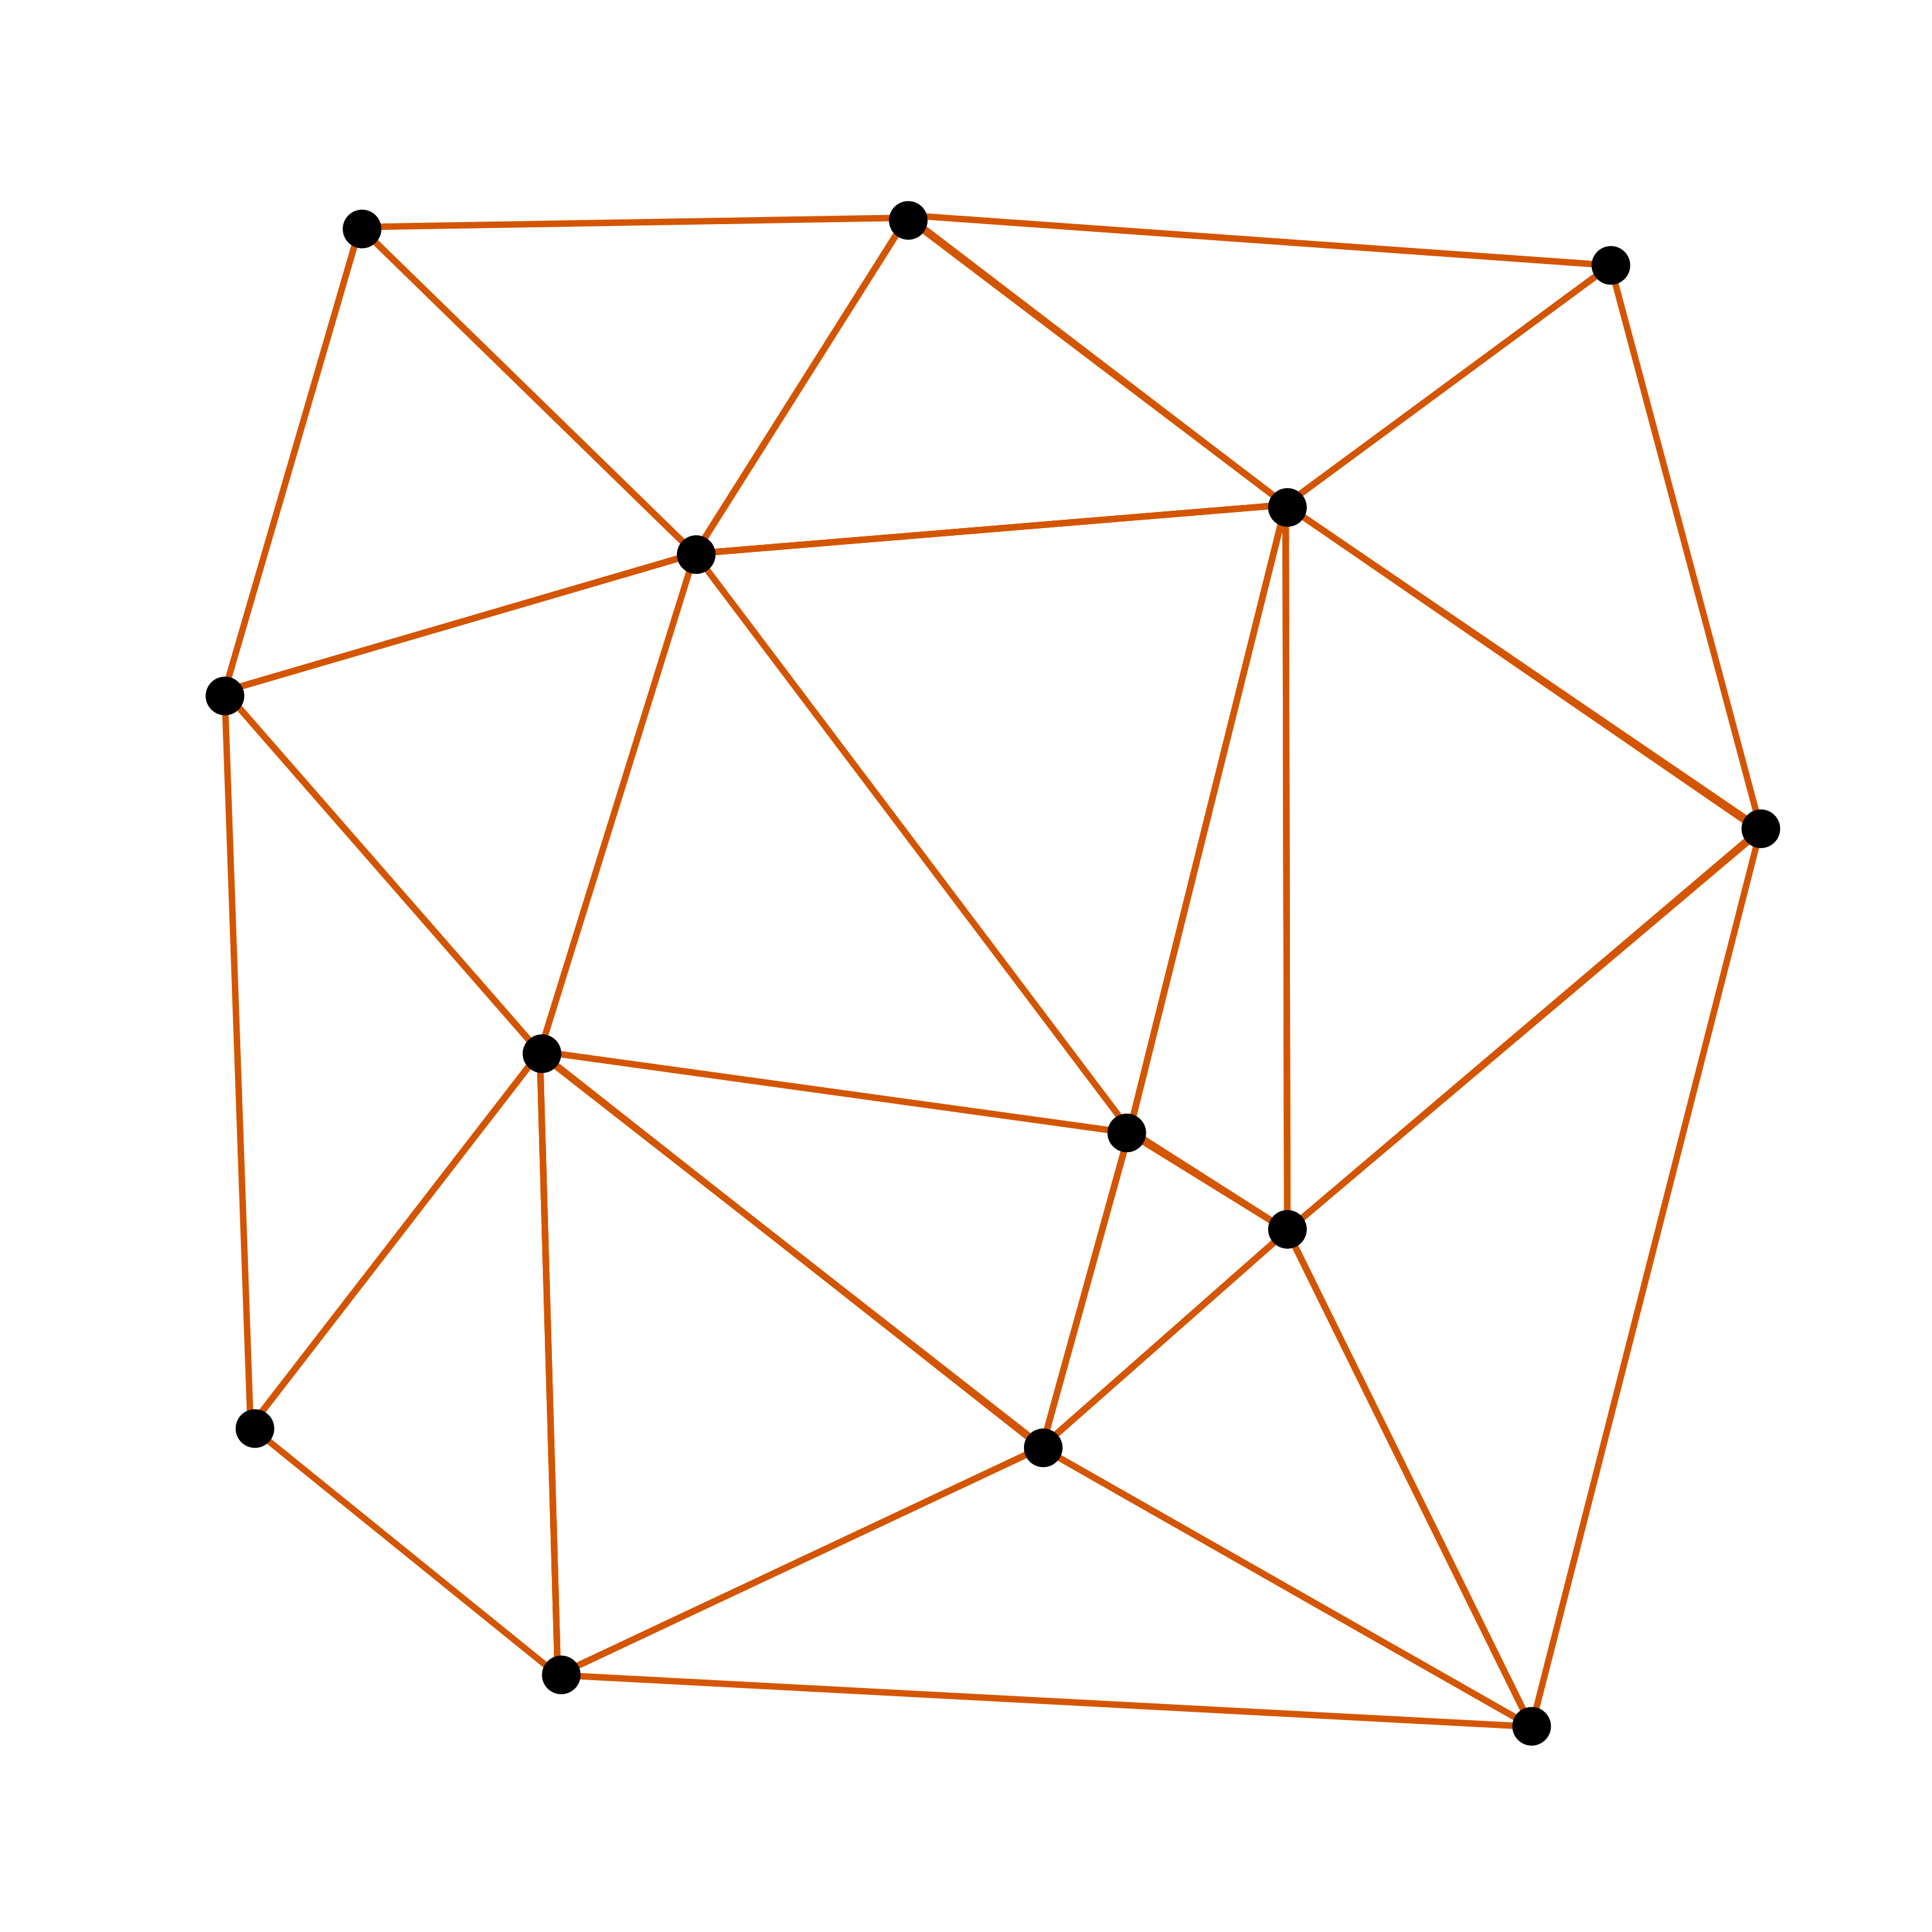
\includegraphics[width=0.4\textwidth]{pictures/Delaunay-Triangulation1.png}

\subsection{Delaunay triangulation}
A delaunay triangulation for a set of points in space is a triangulation of the points, with the added property that no point is inside the circumcircle of any triangle in the triangulation.
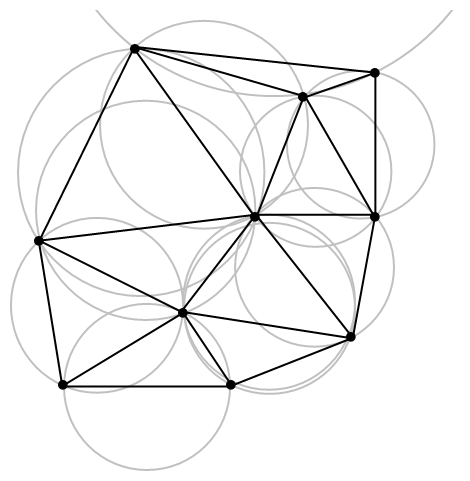
\includegraphics[width=0.4\textwidth]{pictures/Delaunay_circumcircles.png}

The delaunay triangulation is dual to the voronoi diagram.

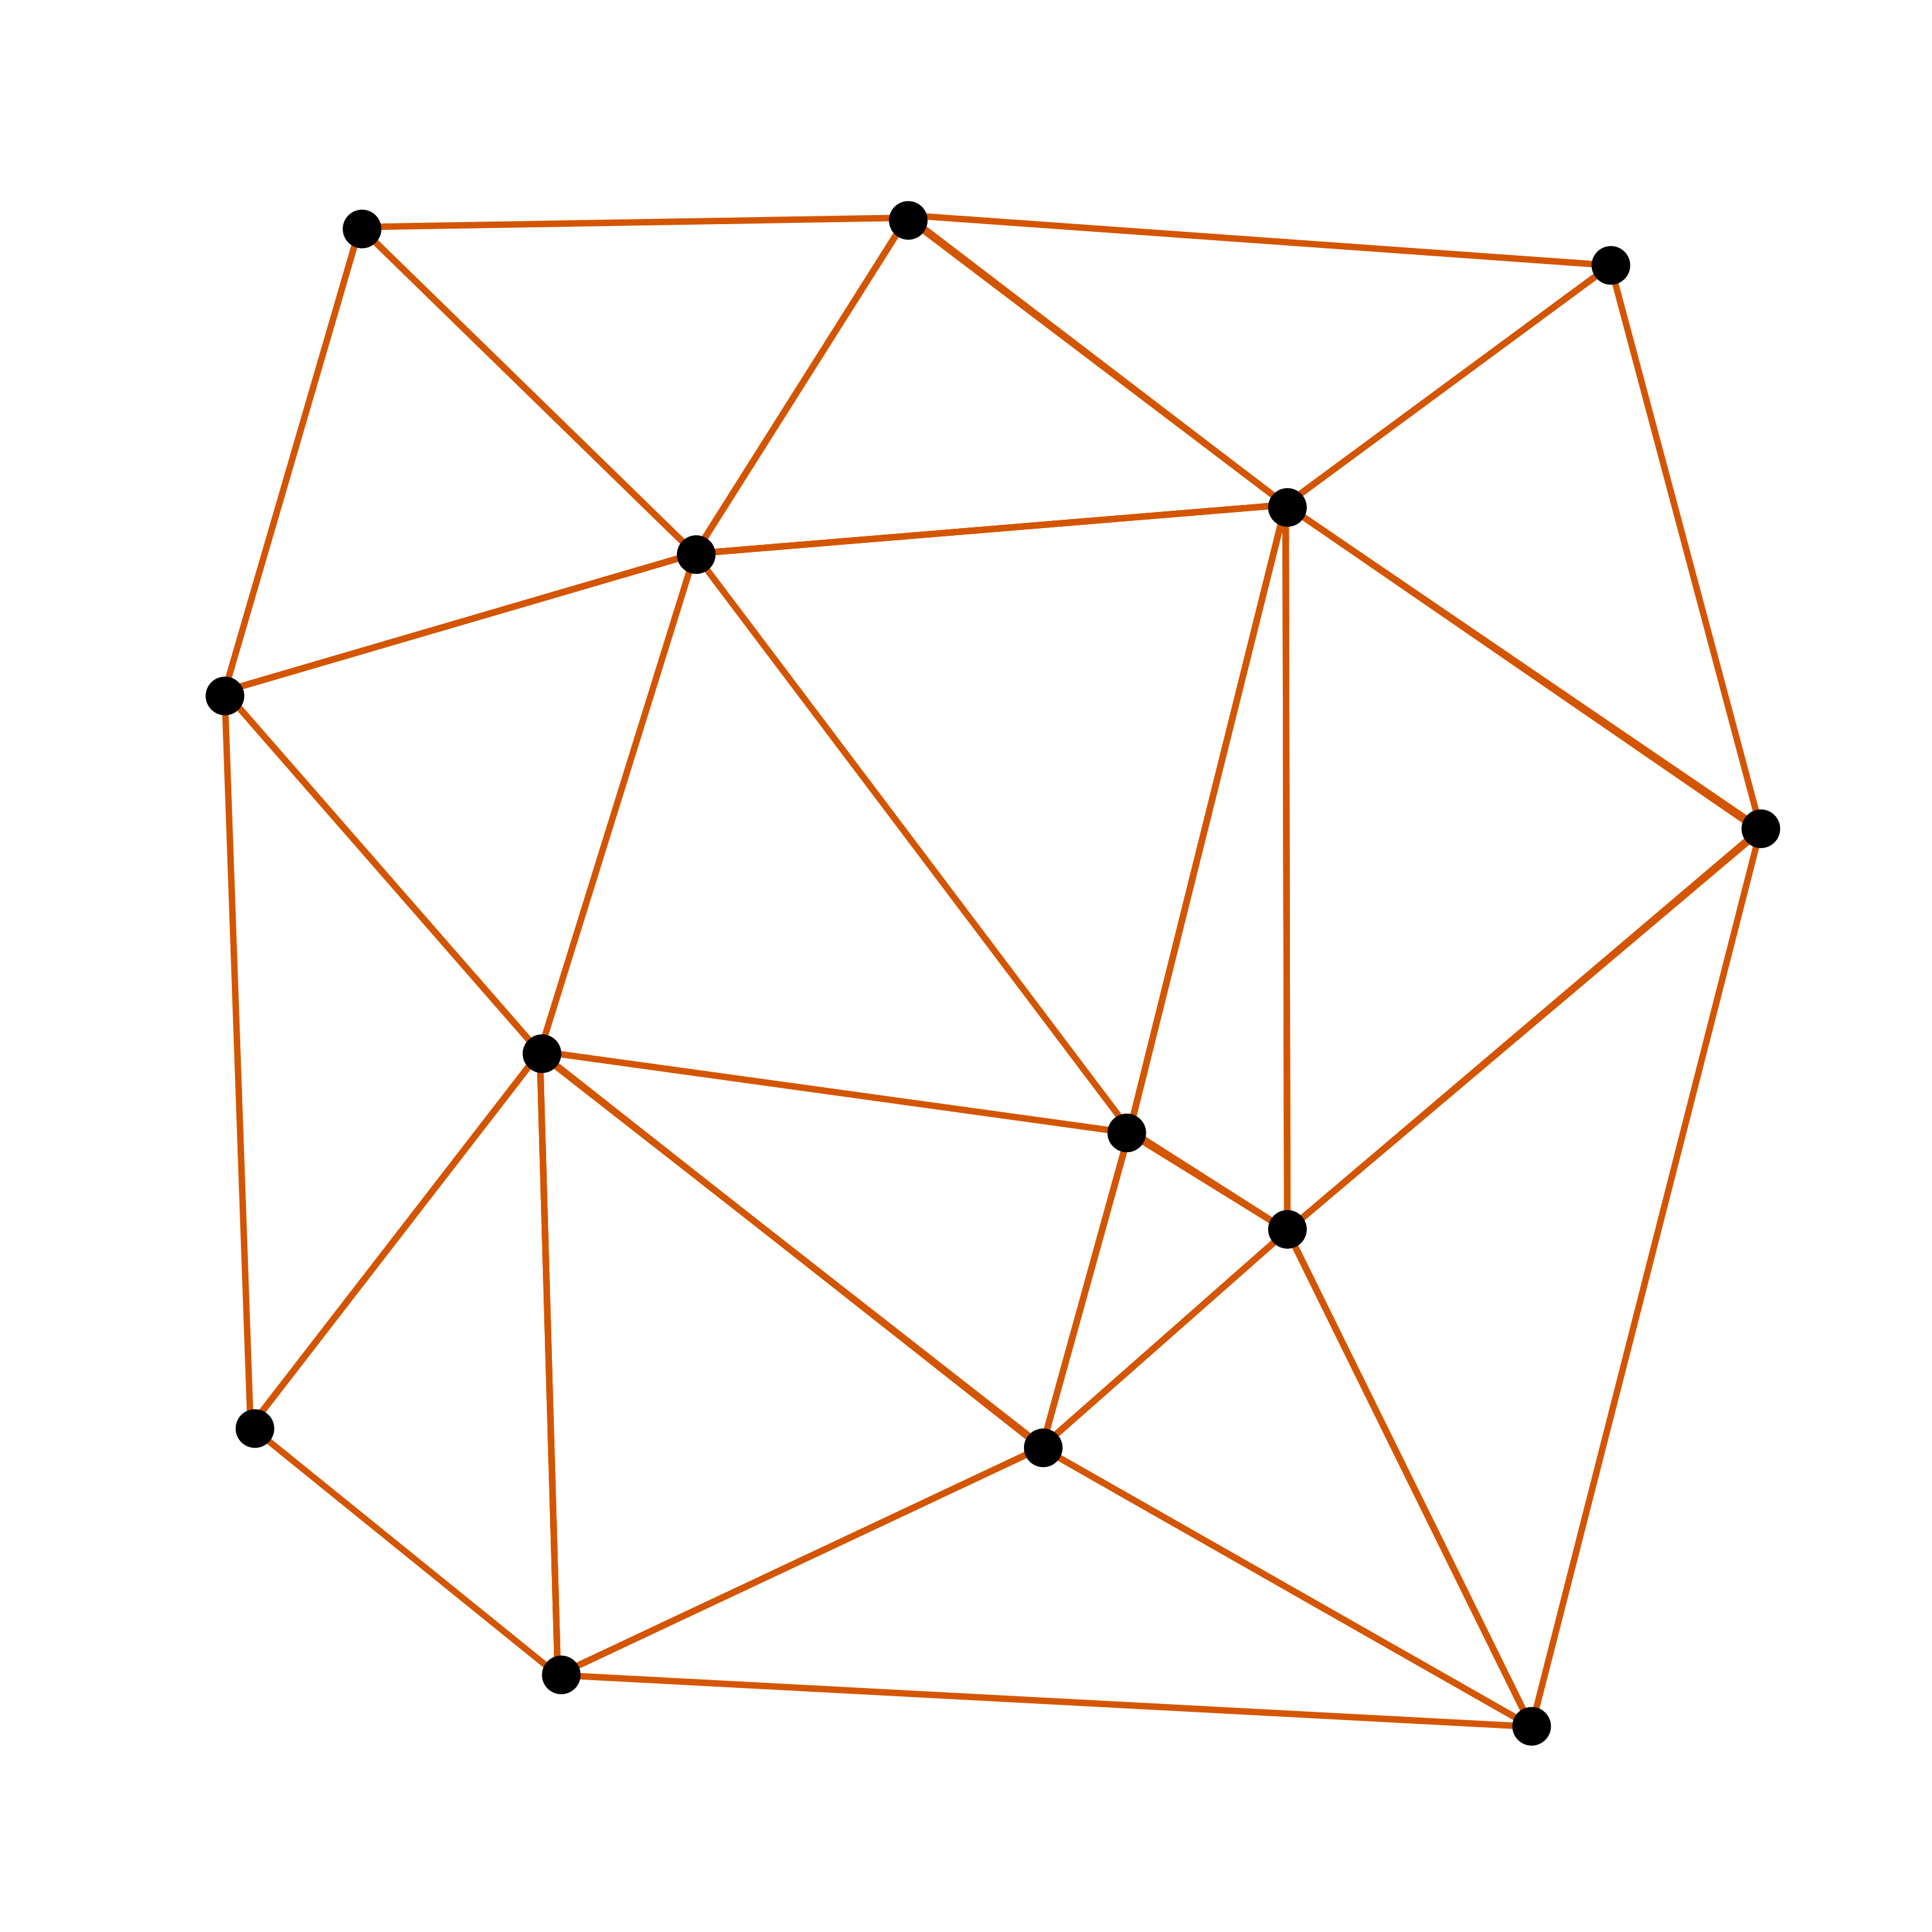
\includegraphics[width=0.3\textwidth]{pictures/Delaunay-Triangulation1.png}
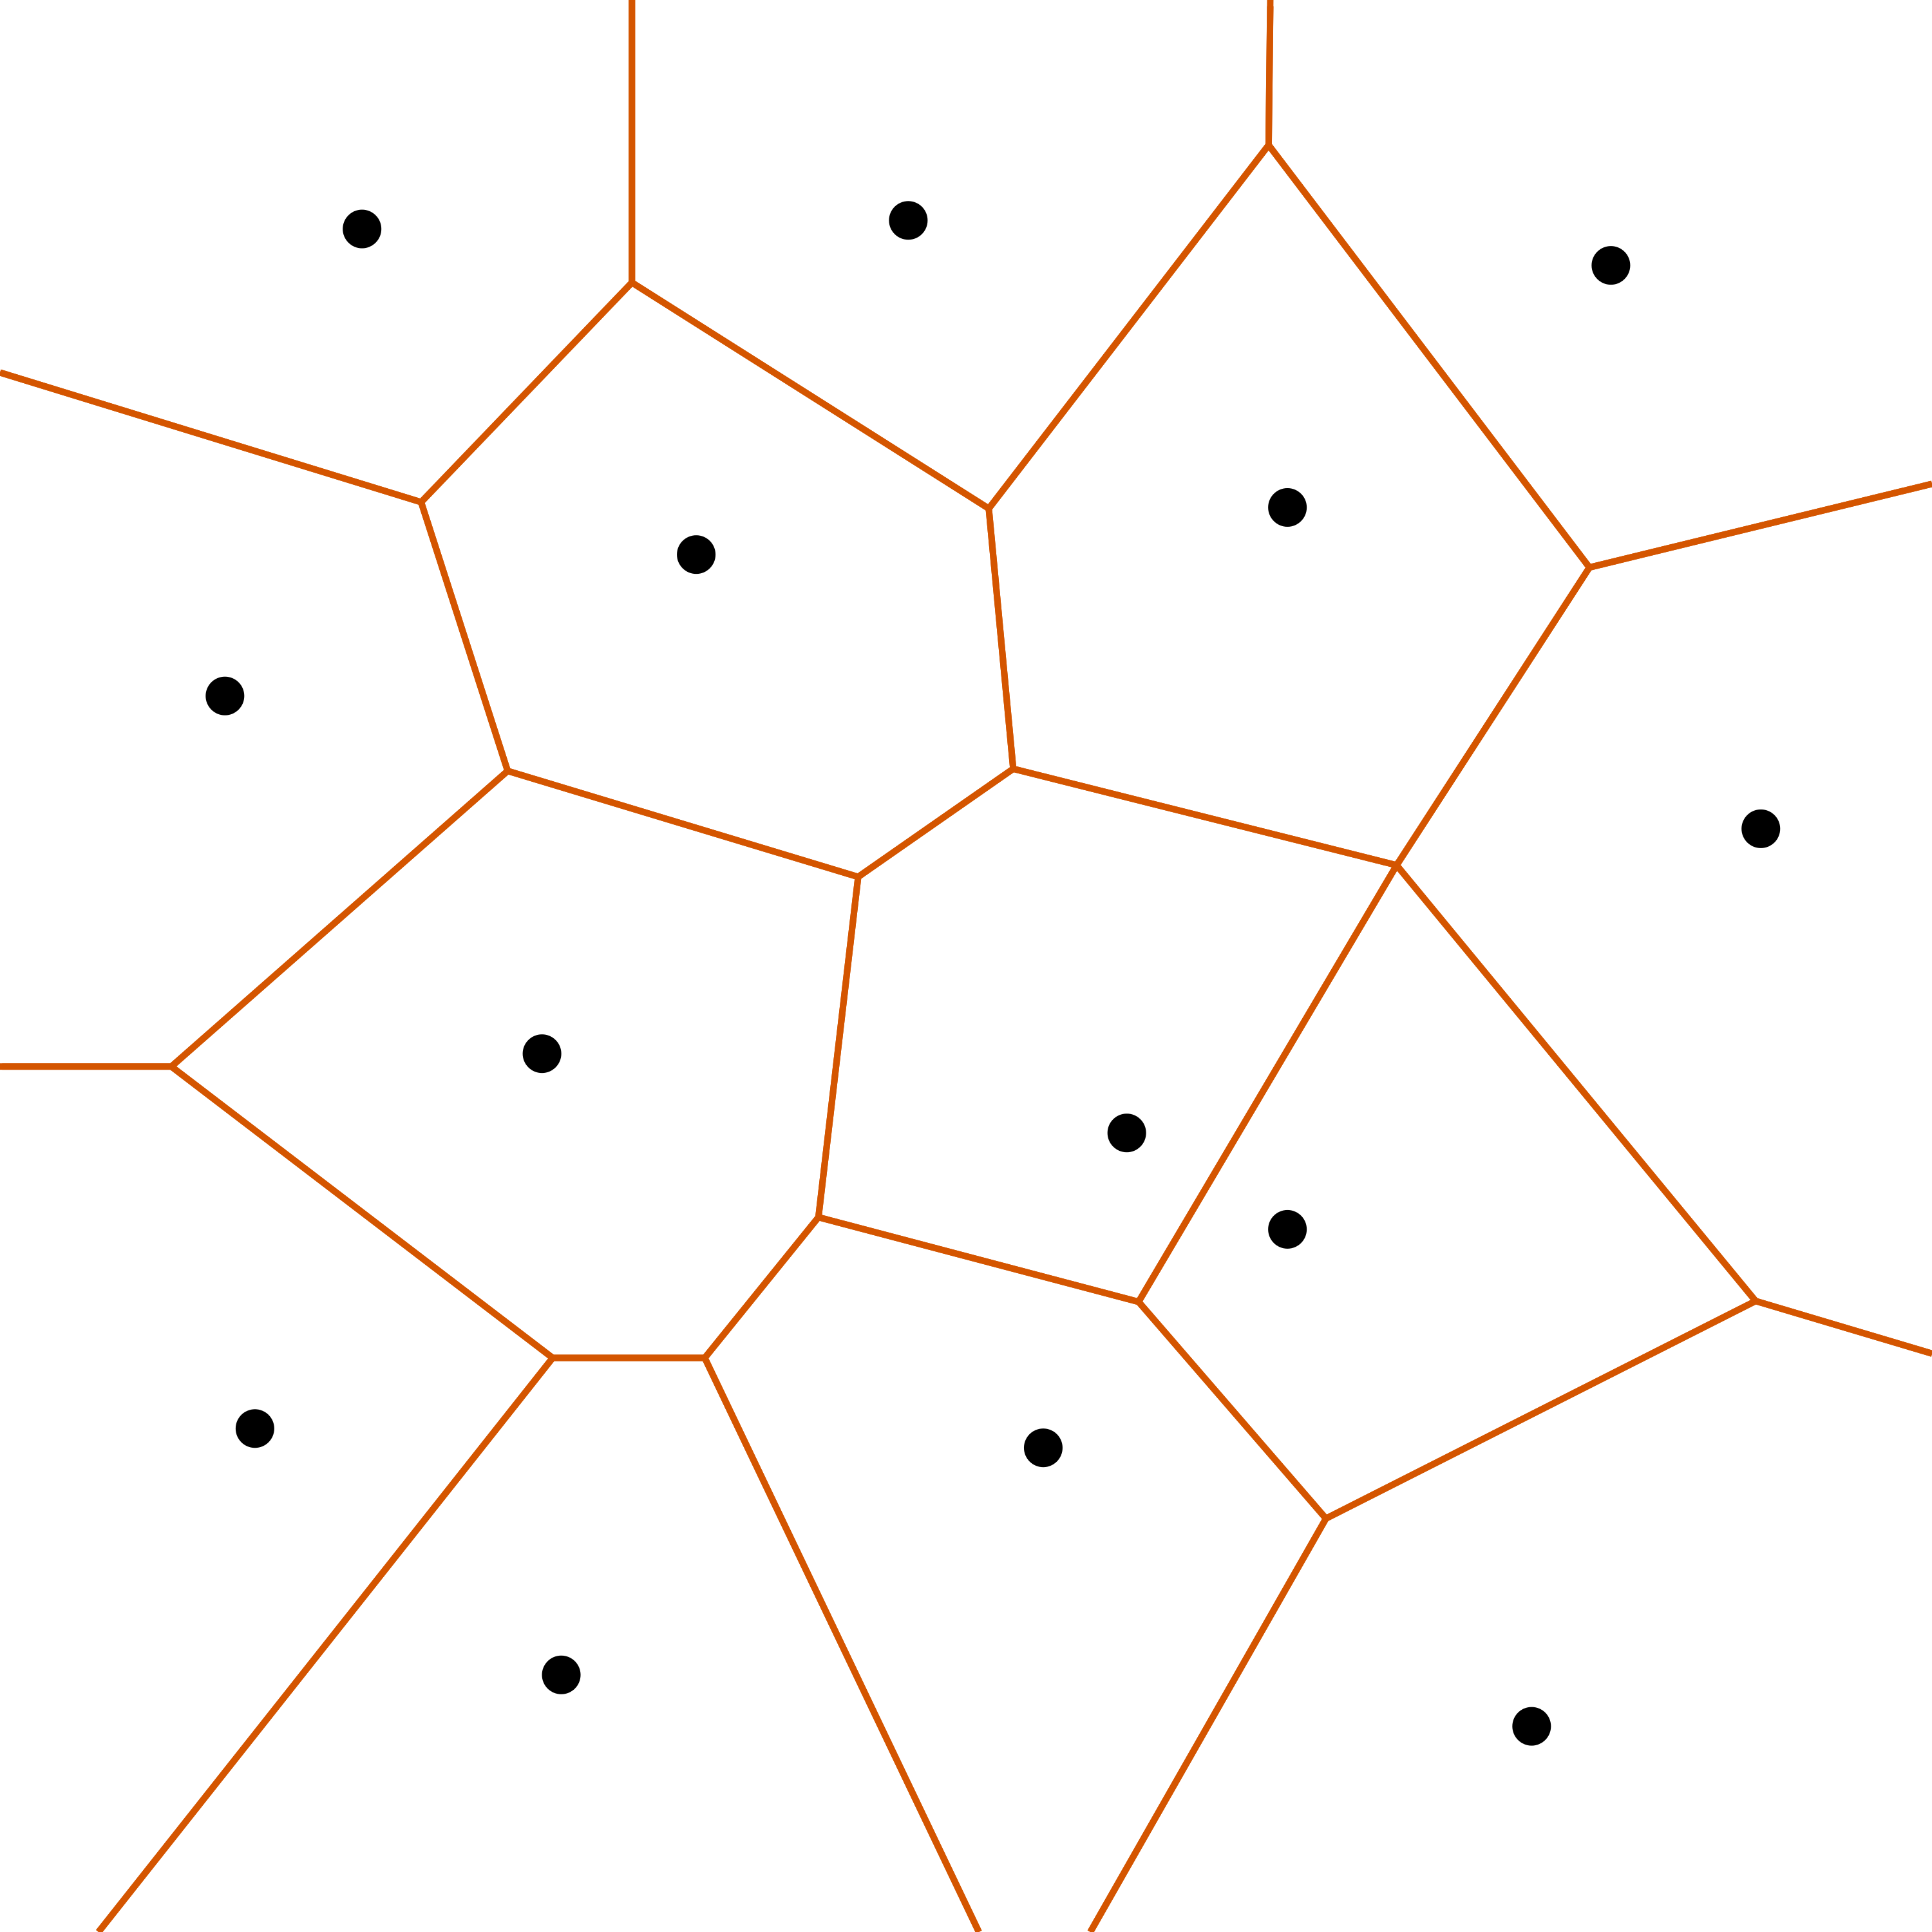
\includegraphics[width=0.3\textwidth]{pictures/Delaunay-Triangulation2.png}
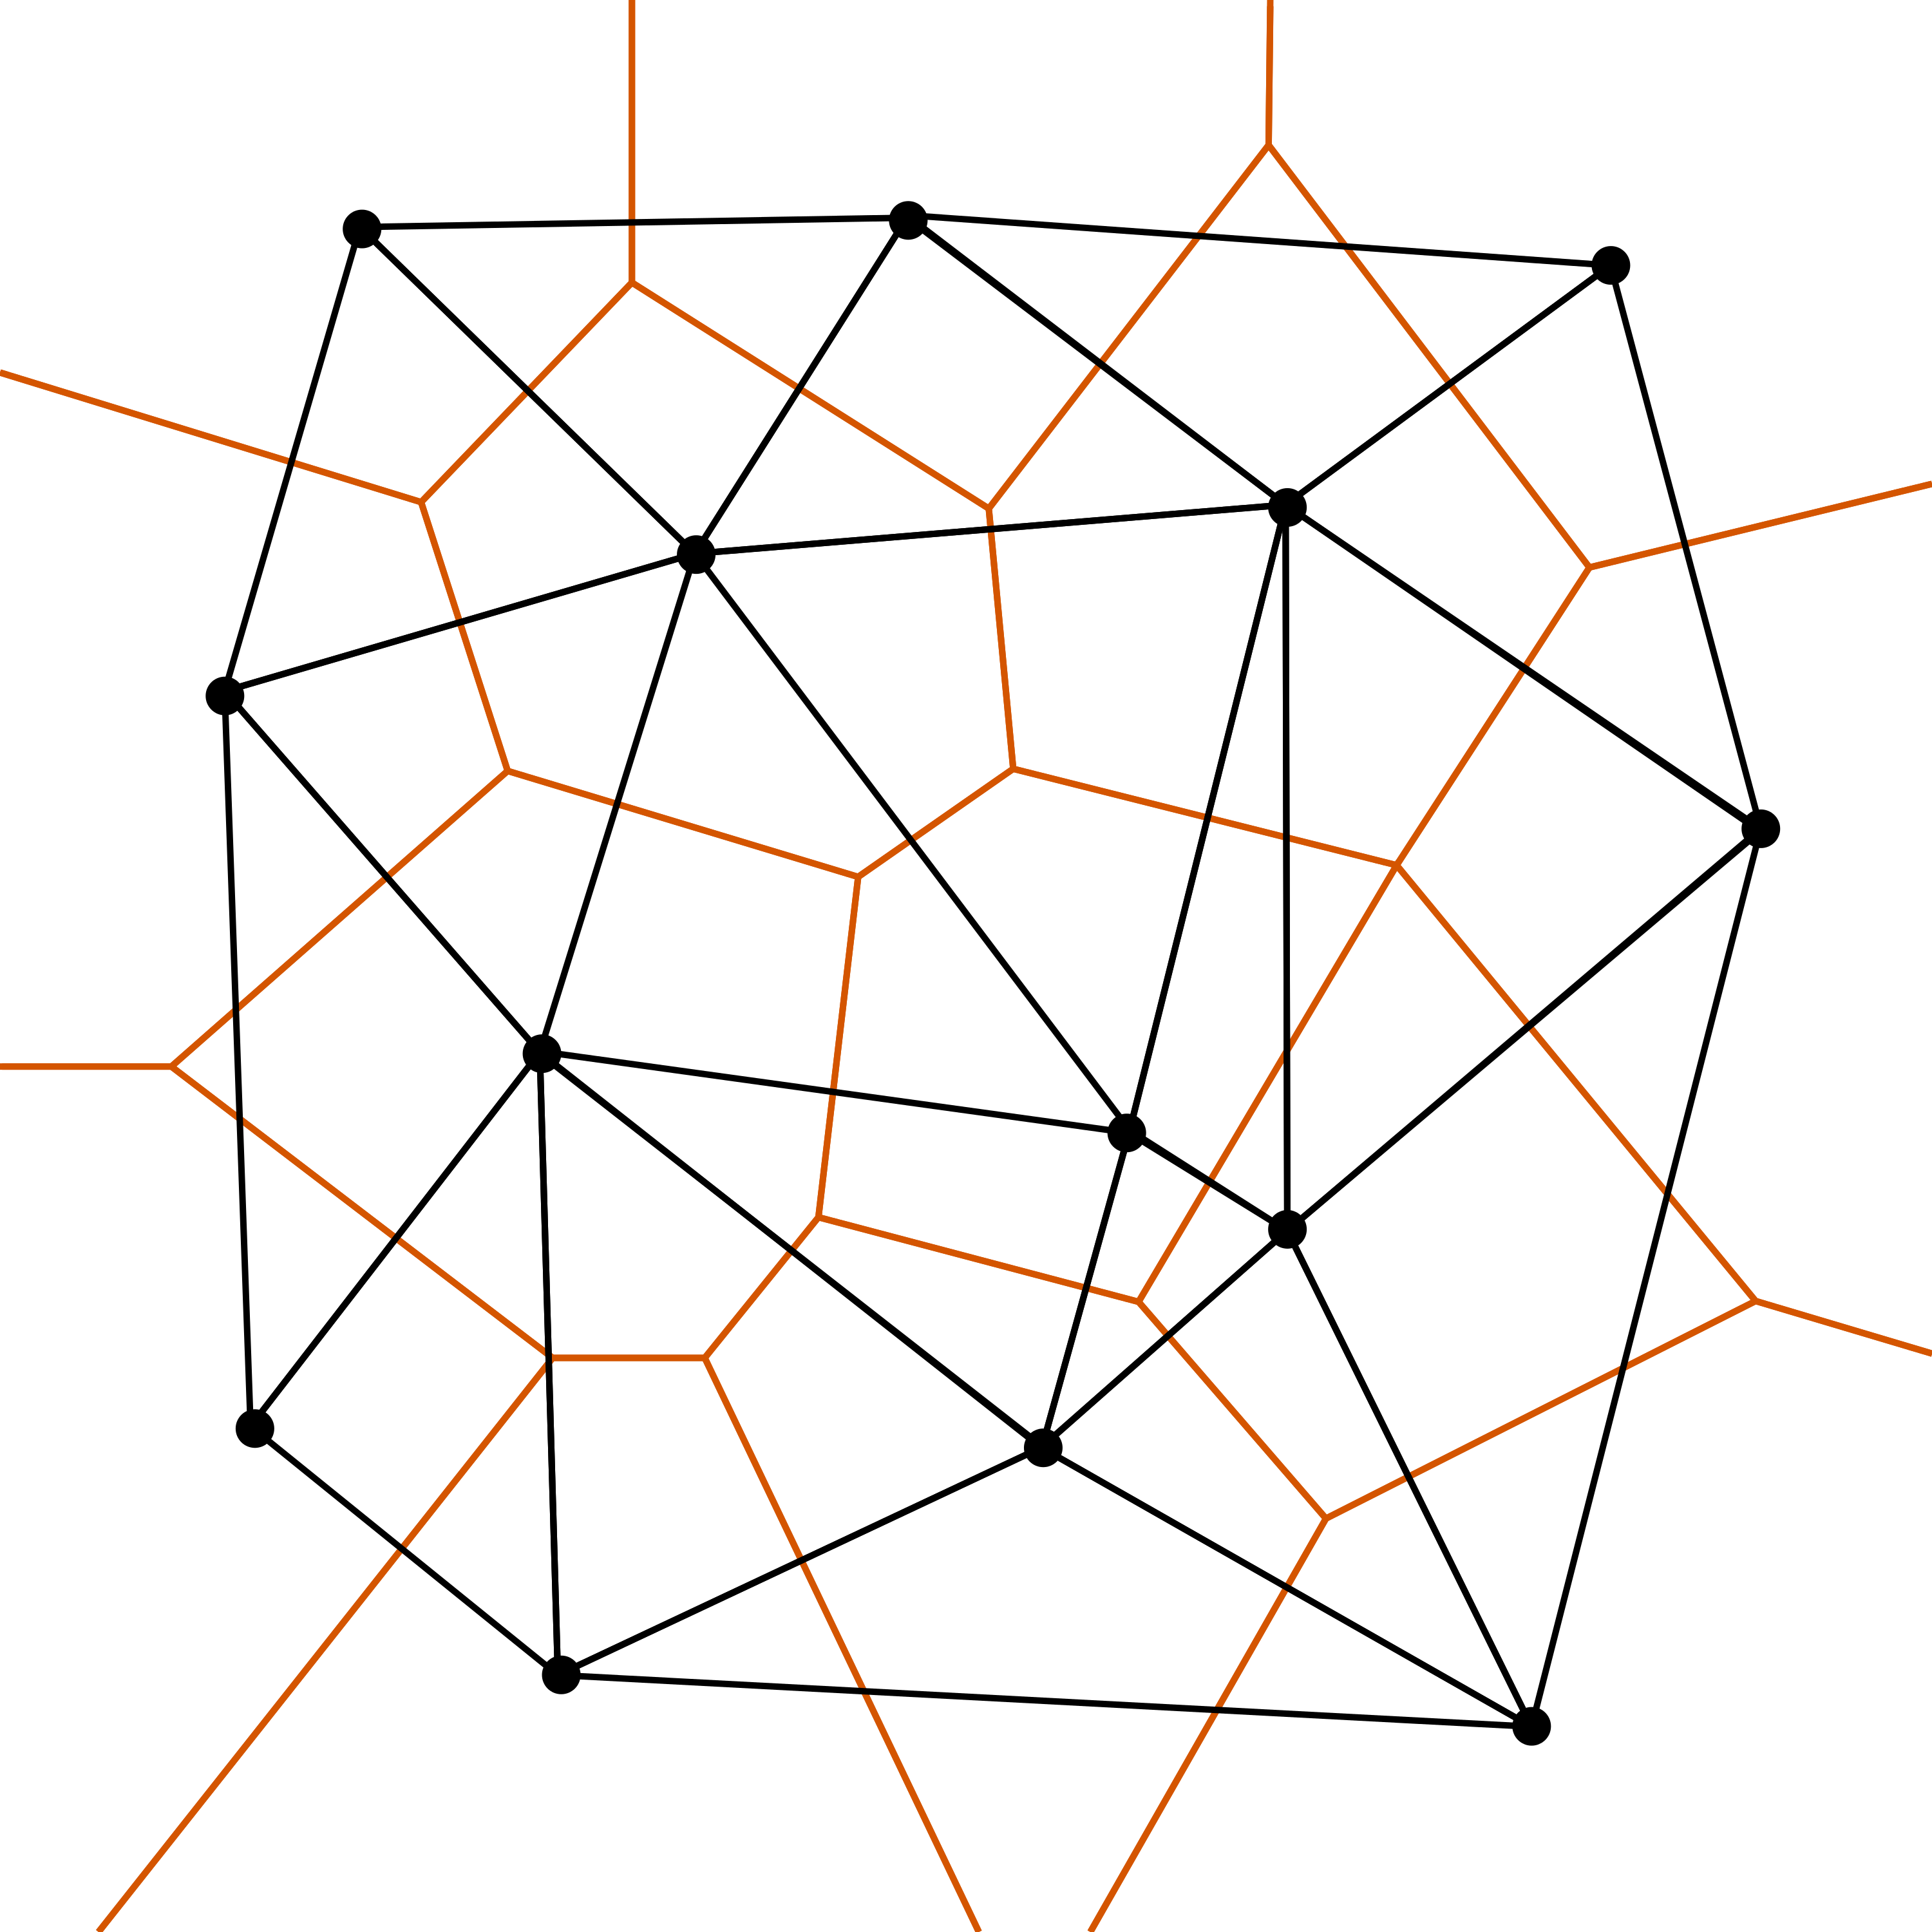
\includegraphics[width=0.3\textwidth]{pictures/Delaunay-Triangulation3.png}

\subsection{Arrangement}
Given a set of planar curves, the arrangement is the subdivision of the plane into zero-dimensional, one-dimensional and two-dimensional cells, called vertices, edges and faces, respectively induced by the given curves.[1 - direct citation]

I don't know what more to say about them. A picture would really just look like any picture :P

\subsection{The Set Cover Problem}
Given a set $\mathcal A$ of sets of numbers, the set cover problem is the problem of finding a minimal subset $\mathcal B$of $\mathcal A$, so that the elements of the union of the sets in $\mathcal B$ is exactly those of the union of the whole of $\mathcal A$.

\subsubsection{example}
Let $\mathcal A$ =  \{\{1,2\}, \{2,3\}, \{2,5\}, \{3,5\}\}. The elements of the union of all sets of $\mathcal A$ is \{1,2,3,5\}. A subset $\mathcal B$ = \{\{1,2\}, \{2,3\}\} has a union \{1,2,3\} and does not cover the set $\mathcal A$. A subset $\mathcal B$ = \{\{1,2\}, \{2,3\}, \{2,5\}\} has a union \{1,2,3,5\} that covers $\mathcal A$, but it is not minimal. A minimal solution is $\mathcal B$ = \{\{1,2\}, \{3,5\}\}.

The set cover problem is known to be NP-complete.[4]
\section{Problem formulation}
Given a set $\mathcal{R}$ of red points, find a set $\mathcal{B}$ of blue points such that in the voronoi diagram of $\mathcal{R} \cup \mathcal{B}$, no two regions corresponding to points in $\mathcal{R}$ are incident to each other. For the delaunay triangulation of $\mathcal{R} \cup \mathcal{B}$, this means that in the triangulation, there is no edge connecting two red points.


\section{Background}
Although not yet shown, the problem is suspected to be NP-hard[2], as a similar problem has been proven to be NP-hard[3].
\subsection{Upper and lower bounds}
Given a set $\mathcal{R}$ of red points, with $|\mathcal{R}| = N$, it has been shown[2] that at least N-1 points are needed to solve this problem. This is exemplified in [REF TO BELOW PICTURE], and always apply to the special case when all points lie in row. In the general case, it has been shown that for $N>2$ there are cases where at least N blue dots are required to solve the problem.

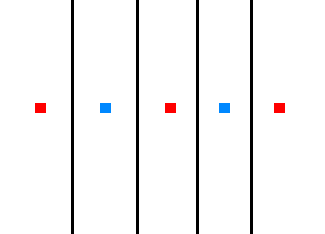
\includegraphics[width=0.3\textwidth]{pictures/N-1solution.png}

In the general case, it has been proved[2] that at most $3N/2$ blue points is needed to solve the problem, and in the case where the points in  $\mathcal{R}$ are in convex position, $5N/2$ points are sufficient. It has been conjectured that $N$ points are sufficient to solve the problem in the general case.

\section{Tools}
\begin{itemize}
\item
Git
\item
Qt
\item
Gurobi
\item
C++
\item
CGAL
\item
CMAKE
\item
GitHub
\end{itemize}


\section{Algorithm outline}
\begin{enumerate}
\item
For the set $\mathcal P$ of points (both red and blue) find the delaunay triangulation.
\item
For each edge connecting two red points in the triangulation, find a circle (REFERENCE DOWN) with the two points on its perimeter and add these to the (possibly empty) set of circles $\mathcal C$.
\item
Calculate the arrangement $\mathcal A$ of the circles $\mathcal C$. (REFERENCE TO INTRODUCTION)
\item
Find a set of points $\mathcal P^*$, so that for every face in the arrangement $\mathcal A$, exactly one point is located in the interior. For every point $\rho  \in \mathcal P^*$ and every circle $\varsigma$ in $\mathcal C$, determine whether $\rho$ is in the interior of $\varsigma$. (REFERENCE DOWN)
\item
Find a minimum subset of $\mathcal P^*$, so that every circle in $\mathcal C$ is covered by at least one point.(REFERENCE DOWN)
\item
Calculate a triangulation for the set of points $\mathcal P^* \cup Red(\mathcal P )$, where  $Red(\mathcal P )$ denotes the set of red points in $\mathcal P$.
\item
If the triangulation contains edges connecting two red points, restart from (2) (MIGHT CHANGE).
\end{enumerate}

\subsection{Finding circles corresponding to unsatisfied edges}

Following the terminology used by the CGAL-project, a \emph{line} is a line unbounded on both sides, whereas an line that is bounded on one side is called a \emph{ray} and when bounded on both sides it is called a \emph{segment}. The approach for choosing circles depends on which type of voronoi edge is to be blocked. Given a voronoi edge, corresponding to the neighbouring points $p_1$ and $p_2$, there are the following cases:

\begin{enumerate}
\item
For a \emph{line}, the smallest possible circle is chosen. This is the circle with its centre in the middle of $p_1$ and $p_2$, and a radius such that $p_1$ and $p_2$ are on its perimeter. A line only occurs in the voronoi diagram in the trivial case where all points lie in a straight line.
\item
For a \emph{ray}, if the point in the middle of $p_1$ and $p_2$ lies on the ray itself, the circle is chosen as for the line. If it is not however, a sufficiently large circle is chosen. Note that a ray in the voronoi diagram is always associated with two points on the convex hull (????????????), for which infinitely large circles exist with the points $p_1$ and $p_2$ on its perimeter.
\item
For a \emph{segment}, the circle with $p_1$ and $p_2$ on its perimeter, and its centre on the middle point of the segment is chosen.
\end{enumerate}

\subsection{Finding a point in the interior of a face}
A relatively difficult task proved to be that of finding a point in the interior of an arbitrary face, given two point $p_1$ and $p_2$ known to be on the boundary of the face. The following algorithm was used.

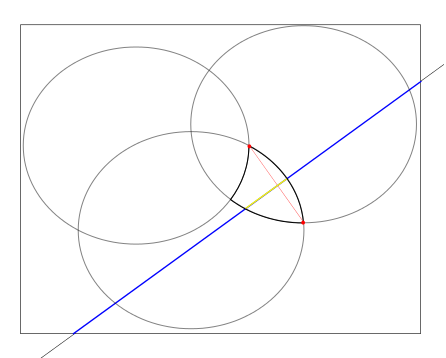
\includegraphics[width=0.4\textwidth]{pictures/PointInFace.png}
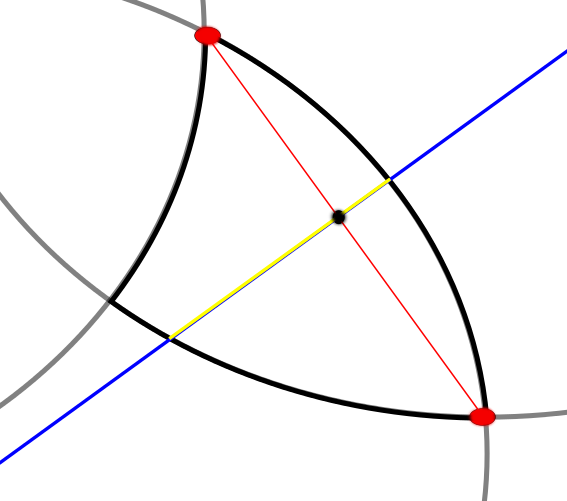
\includegraphics[width=0.3\textwidth]{pictures/PointInFace2.png}

\begin {itemize}
\item
Find the point $p_m$ in the middle of $p_1$ and $p_2$. If this point is inside the face, chose this point. (WE DON'T ACTUALLY DO THIS YET)
\item
Find the line $l$ going through $p_m$ and is perpendicular to the edge between $p_1$ and $p_2$.
\item
Find the segment $s$ that is the intersection of $l$ and the smallest rectangle large enough to contain all circles of the arrangement. This step is needed because a CGAL function needs an object of type segment as input. We describe this step here for the sake of completeness.
\item
Find the segment that is the intersection of the segment $s$ and the face itself.
\item
Any point except the endpoints of this segment are inside the face. The midpoint of the segment is chosen.
\end{itemize}

\subsection{Finding a minimal subset of points}
The problem of finding a minimal subset of a set of points $\mathcal P^*$, so that at least one point in $\mathcal P$ is in the interior of each circle in $\mathcal C$, is exactly that of the set covering problem. (SHOULD WE GIVE AN EXAMPLE, SHOWING THAT THEY LOOK ALIKE?). The problem is easily stated in terms of an integer programming problem, and can thus be solved relatively efficiently with an integer programming solver, such as Gurobi.
\subsubsection{Pseudo code }
For every point $\rho_i \in \mathcal P^*$, let $x(\rho_i)$ be a boolean, set to 1 if the point $\rho_i$ appears in a solution and 0 otherwise. Also, for every circle $\varsigma_j \in \mathcal C$, let $\varsigma_j (\rho_i)$ be 1 if point $\rho_i$ lies in the interior of $c_j$ and 0 otherwise.



\begin{lstlisting}[mathescape]
Minimize: $\sum\limits_{ \rho \in \mathcal P^*} x(\rho_{i}) \hspace{70pt} $
Constraint: $\sum\limits_{ \rho \in \mathcal P^*} \varsigma_j(\rho_i) \geq 1 \hspace{40pt}$ for each $\varsigma \in \mathcal C$
\end{lstlisting}

\section{Just to remember}
\begin{itemize}
\item
A graphical gui for input, with input of red dots either by manual placement or by reading a file
\item
Output by drawing delaunay circles and voronoi-edges.
The Arrangement can also be saved to a file (saving the points is sufficient).

\end{itemize}


\section{Abstract program layout}
How are the different parts of the program put together. Right now, we basically have a CGAL-part, a QT-part and a gurobi-part. Then we have one class, Geometry, that puts them all together. This is actually quite good.

We also have the file myGraphics.cpp, which uses CGAL directly. We should probably avoid this, and use functions in Geometry.cpp instead.
I didn't find where myGraphics uses CGAL directly. Do you mean that myGraphics calls functions of CGAL-Objects, like in "circs.back().squared\_radius()" ?
If so, I think you're theoretically right and we should avoid this in favor of a better structure, but I think it's not important enough to spend time doing this, and more important, changing this might decrease performance.

A picture showing file dependencies would be nice.

\section{Problems encountered}
\begin{itemize}
\item
Getting all the different parts (tools) to work and compile together. Especially cmake. Gurobi could also be mentioned, as it needs a C++ wrapper or whatever you call it.
\item
Finding a point inside a face. If we end up using the algorithm we have now, that algorithm would need a quite nice picture. And pictures are nice.
\item
Hopefully nothing more, but I don't think we will be that lucky :)
\end{itemize}
\section{Results}
What did we manage to do. What didn't we manage to do. This is a little bit difficult to outline at this stage.

\section{Result}
\begin{itemize}
\item
A picture of the gui
\item
Some problems, and the resulting solution.
\item
How well does it perform?
\end{itemize}

\section{Discussion}
Even more difficult at this stage


\section{references}
Keeping the references I used in the last project, since they probably follow a good convention.

[1] H. G. Cobb, J. J. Grefenstette (1993)

Genetic Algorithms for Tracking Changing Environments

Proceedings of the 5th International Conference on Genetic Algorithms

[2] A. Simões, E. Costa (2002)

Using Genetic Algorithms to Deal with Dynamic Environments: A Comparative Study of Several Approaches Based on Promoting Diversity

GECCO '02 Proceedings of the Genetic and Evolutionary Computation Conference

[3] S. Yang (2007)

Genetic Algorithms with Elitism-Based Immigrants for Changing Optimization Problems

Lecture Notes In Computer Science, 2007, volume 4448, pages 627-636

-----------------------------------------

[1]

http://www.cgal.org/Manual/3.3/doc\_html/cgal\_manual/Arrangement\_2/Chapter\_main.html

[2] O. Aichholzer, R. Fabila-Monroy, T. Hackl, M. van Kreveld, A. Pilz, P. Ramos, und B. Vogtenhuber

Blocking Delaunay Triangulations. 

Proc. Canadian Conference on Computational Geometry, CCCG 2010, Winnipeg, August 9­11, 2010. 

% NP-hardness of a similar problem
[3] M. de Berg, D. Gerrits, A. Khosravi, I. Rutter, C. Tsirogiannis and A. Wolff.

How Alexander the Great Brought the Greeks Together while Inflicting Minimal Damage to the Barbarians.

Proc. 26th European Workshop on Computational Geometry, pages 73–76, 2010.

[4] Richard M. Karp
Reducibility Among Combinatorial Problems.
In: R. E. Miller, J. W. Thatcher (Hrsg.): Complexity of Computer Computations. Plenum Press, New York 1972, S. 85–103.

-----------------------------------------


Delaunay circumcircles, GNU Free Documenation Licence, Nü es

http://commons.wikimedia.org/wiki/File:Delaunay\_circumcircles.png


Delaunay triangulation 1-3, public domain, user Capheiden 

http://upload.wikimedia.org/wikipedia/de/1/17/Voronoi-Delaunay.svg

http://upload.wikimedia.org/wikipedia/de/4/48/Voronoi-Diagramm.svg

http://upload.wikimedia.org/wikipedia/commons/1/1f/Delaunay-Triangulation.svg

\end{document}

